\chapter{\IfLanguageName{dutch}{Stand van zaken}{State of the art}}%
\label{ch:stand-van-zaken}

% Tip: Begin elk hoofdstuk met een paragraaf inleiding die beschrijft hoe
% dit hoofdstuk past binnen het geheel van de bachelorproef. Geef in het
% bijzonder aan wat de link is met het vorige en volgende hoofdstuk.

% Pas na deze inleidende paragraaf komt de eerste sectiehoofding.

% Dit hoofdstuk bevat je literatuurstudie. De inhoud gaat verder op de inleiding, maar zal het onderwerp van de bachelorproef *diepgaand* uitspitten. De bedoeling is dat de lezer na lezing van dit hoofdstuk helemaal op de hoogte is van de huidige stand van zaken (state-of-the-art) in het onderzoeksdomein. Iemand die niet vertrouwd is met het onderwerp, weet nu voldoende om de rest van het verhaal te kunnen volgen, zonder dat die er nog andere informatie moet over opzoeken \autocite{Pollefliet2011}.

% Je verwijst bij elke bewering die je doet, vakterm die je introduceert, enz.\ naar je bronnen. In \LaTeX{} kan dat met het commando \texttt{$\backslash${textcite\{\}}} of \texttt{$\backslash${autocite\{\}}}. Als argument van het commando geef je de ``sleutel'' van een ``record'' in een bibliografische databank in het Bib\LaTeX{}-formaat (een tekstbestand). Als je expliciet naar de auteur verwijst in de zin (narratieve referentie), gebruik je \texttt{$\backslash${}textcite\{\}}. Soms is de auteursnaam niet expliciet een onderdeel van de zin, dan gebruik je \texttt{$\backslash${}autocite\{\}} (referentie tussen haakjes). Dit gebruik je bv.~bij een citaat, of om in het bijschrift van een overgenomen afbeelding, broncode, tabel, enz. te verwijzen naar de bron. In de volgende paragraaf een voorbeeld van elk.

% \textcite{Knuth1998} schreef een van de standaardwerken over sorteer- en zoekalgoritmen. Experten zijn het erover eens dat cloud computing een interessante opportuniteit vormen, zowel voor gebruikers als voor dienstverleners op vlak van informatietechnologie~\autocite{Creeger2009}.

% Let er ook op: het \texttt{cite}-commando voor de punt, dus binnen de zin. Je verwijst meteen naar een bron in de eerste zin die erop gebaseerd is, dus niet pas op het einde van een paragraaf.

\label{sec:grafiekmodellering}
\section{Grafiekmodellering}
Grafiekmodellering is een techniek die gebruikt wordt om data te visualiseren en te analyseren. Dit gebeurt door middel van knopen die verbonden zijn met edges, welke de relaties tussen de verschillende knopen weergeven \autocite{neo4j2025}.
Een knoop stelt een entiteit voor, zoals een persoon, een product of een proces. Een edge stelt de relatie tussen de verschillende knopen voor zoals een associatie, transformatie of transactie van een product.
Dit kan in ons geval een staalplaat zijn die door een kraan verplaatst wordt. Hierbij zijn de kraan en staalplaat de knopen en is de verplaatsing een transactie-relatie tussen deze knopen.
Elke knoop bevat ook properties die de knoop beschrijven. Dit kan bijvoorbeeld het bouwjaar van een machine zijn of de temperatuur van een product, deze worden opgeslagen als key-value paar om later efficiënt te kunnen ophalen.

\subsection{Cosmos DB}%
Cosmos DB is een NoSQL\-database van Microsoft. Het biedt een lage latentie, multi\-query-API die eenvoudig grote hoeveelheden data kan verwerken en heeft een grote beschikbaarheid zegt~\textcite{Put2020}, wat zeer belangrijk is in ons project.
Daarnaast is CosmosDB horizontaal schaalbaar, wat betekent dat we op hoogtepunten tot een miljoen lees- en schrijfaanvragen kunnen verwerken door het benodigde aantal servers toe te voegen.
De hoge beschikbaarheid wordt gegarandeerd door replicatie, waardoor we snel kunnen overschakelen als er een probleem is in onze database.

\subsection{Gremlin API}
Gremlin is een database query taal die gebruikt wordt om te communiceren met grafiek databases zoals CosmosDB \autocite{Tinkerpop2023}.\@
De taal bevat verschillende varianten zoals Gremlin-Java, Gremlin-Python en Gremlin-Groovy,\dots
In ons geval zullen we Gremlin-Javascript gebruiken om de data van ArcelorMittal Gent in CosmosDB te bevragen. De bevraging is gebasseerd op een RestAPI die de data ophaalt en teruggeeft in json formaat.
Javascript is hiervoor geschikt omdat Javascript en json een goede combinatie zijn om data te verwerken, daarnaast maken we ook gebruik van nodejs wat met javascript werkt. 
Als extra kan je met javascript eenvoudig front end en back end combineren, wat mogelijk is voor verdere uitbereiding van deze thesis.

\subsection{NodeJS}
NodeJS is een open-source JavaScript runtime-omgeving die de mogelijkheid biedt om JavaScript-code uit te voeren op de server \autocite{NodeJS2022}.
Dit gebeurt Single\-Threaded, Non\-Blocking I/O model wat betekent dat er geen nieuwe threads worden aangemaakt voor elke request.
Door middel van Callbacks en Promises werkt nodejs asynchroon, wat betekent dat de code niet wacht op een antwoord van een request maar ondertussen andere requests kan verwerken.
Met event loops worden de requests in een wachtrij geplaatst en worden ze verwerkt wanneer de server klaar is met een andere operatie.
Daardoor is NodeJS zeer performant en schaalbaar voor het verwerken van grote hoeveelheden data.

De tecnologie is in 2009 ontwikkeld en geintroceerd door Ryan Dahl en is sindsdien zeer populair geworden in de webontwikkeling. 
NodeJS is later door grote bedrijven zoals Netfilx, eBay \& Uber gebruikt voor hun back-end systemen.
Zoals eerder vermeld is het geen framework maar een runtime-omgeving, dit betekent dat het geen standaardbibliotheken heeft die hergebruikt kunnen worden door developers.
Daardoor ben je volledig vrij in hoe je de architectuur van je applicatie opbouwt.

Een van de nadelen van nodejs is dat het single\-threaded is, wat betekent dat het niet geschikt is voor CPU-intensieve taken.
Dit komt omdat nodejs gebruik maakt van een event loop die de requests in een wachtrij plaatst en ze verwerkt wanneer de server klaar is met een andere operatie.
Hierdoor kan het zijn dat een request die veel tijd nodig heeft om te verwerken de andere requests blokkeert.
Sinds 2018 is er een nieuwe feature geïntroduceerd in nodejs genaamd Worker Threads, dit maakt het mogelijk om multi\-threaded te werken in nodejs.
Daardoor kunnen we de CPU\-intensieve taken in een aparte thread verwerken en de main thread vrij houden voor andere requests.

\subsection{EPCIS}
Voor dit onderzoek moet alles voldoen aan de EPCIS (Electronic Product Code Information Services) waarden, dit zijn de wat, wanneer, waar, waarom en hoe. 
Deze waarden zijn ontwikkeld door GS1 om gegevens over beweging, status en verandering van een item in de toeleveringsketen (supply chain) vast te leggen en te delen binnen en buiten het bedrijf \autocite{Devins}.
``Met behulp van deze waarden kunnen we real-life objecten omzetten in elektronisch opgeslagen informatie, waarna we dit kunnen communiceren met eindgebruikers.`` zegt \textcite{Devins}.
Door deze normen toe te passen kunnen we de traceerbaarheid van het product per proces garanderen inclusief de gewenste parameters die opgeslagen worden in ons grafiekmodel zoals tijd (wanneer) en temperatuur (hoe) waar nodig.
\bigbreak
EPCIS is een GS1-standaard die bedrijven in staat stelt om gebeurtenissen in de toeleveringsketen vast te leggen en te delen. Het biedt een gemeenschappelijk kader voor het vastleggen van de wat, wanneer, waar en waarom van gebeurtenissen die betrekking hebben op fysieke of digitale objecten. Dit helpt bedrijven om een gedetailleerd overzicht te krijgen van de bewegingen en status van producten in de toeleveringsketen, wat essentieel is voor traceerbaarheid en transparantie.

Volgens GS1 \autocite{GS12025} zijn de belangrijkste voordelen van EPCIS:
\begin{table}[H]
    \centering
     \begin{tabular}{lp{0.6\textwidth}}
          \toprule
          \textbf{Voordeel} & \textbf{Beschrijving} \\
          \toprule
          Verbeterde zichtbaarheid & Door het vastleggen en delen van gedetailleerde gebeurtenisgegevens kunnen bedrijven beter inzicht krijgen in de bewegingen en status van producten in de toeleveringsketen. \\
          \midrule
          Efficiëntieverbeteringen & Door het automatiseren van gegevensverzameling en -uitwisseling kunnen bedrijven operationele efficiëntie verbeteren en fouten verminderen. \\
          \midrule
          Naleving van regelgeving & EPCIS helpt bedrijven te voldoen aan wettelijke vereisten voor traceerbaarheid en rapportage. \\
          \midrule
          Betere samenwerking & Door het delen van gebeurtenisgegevens met handelspartners kunnen bedrijven beter samenwerken en de toeleveringsketen optimaliseren. \\
          \bottomrule
     \end{tabular}
     \caption[Belangrijkste voordelen van EPCIS volgens GS1]{\label{tab:epcis-voordelen}}
\end{table}

Door EPCIS te implementeren in ons project kunnen we ervoor zorgen dat alle relevante gegevens over de beweging en status van producten nauwkeurig worden vastgelegd en gedeeld, wat bijdraagt aan een efficiëntere en transparantere toeleveringsketen.

% \begin{figure}
%   \centering
%   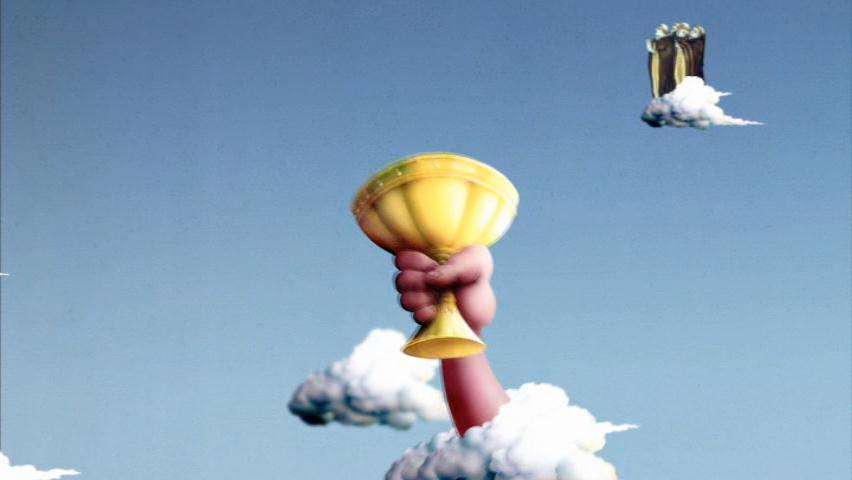
\includegraphics[width=0.8\textwidth]{grail.jpg}
%   \caption[Voorbeeld figuur.]{\label{fig:grail}Voorbeeld van invoegen van een figuur. Zorg altijd voor een uitgebreid bijschrift dat de figuur volledig beschrijft zonder in de tekst te moeten gaan zoeken. Vergeet ook je bronvermelding niet!}
% \end{figure}

% \begin{listing}
%   \begin{minted}{python}
%     import pandas as pd
%     import seaborn as sns

%     penguins = sns.load_dataset('penguins')
%     sns.relplot(data=penguins, x="flipper_length_mm", y="bill_length_mm", hue="species")
%   \end{minted}
%   \caption[Voorbeeld codefragment]{Voorbeeld van het invoegen van een codefragment.}
% \end{listing}


% \begin{table}
%   \centering
%   \begin{tabular}{lcr}
%     \toprule
%     \textbf{Kolom 1} & \textbf{Kolom 2} & \textbf{Kolom 3} \\
%     $\alpha$         & $\beta$          & $\gamma$         \\
%     \midrule
%     A                & 10.230           & a                \\
%     B                & 45.678           & b                \\
%     C                & 99.987           & c                \\
%     \bottomrule
%   \end{tabular}
%   \caption[Voorbeeld tabel]{\label{tab:example}Voorbeeld van een tabel.}
% \end{table}

